\section{Dini Permata Putri (1174053)}
\subsection{Menulis Shapefile}

\begin{enumerate}
	\item Nomor 1
	\lstinputlisting{src/tugas2/1174053/No1.py}
	\begin{figure}[H]
		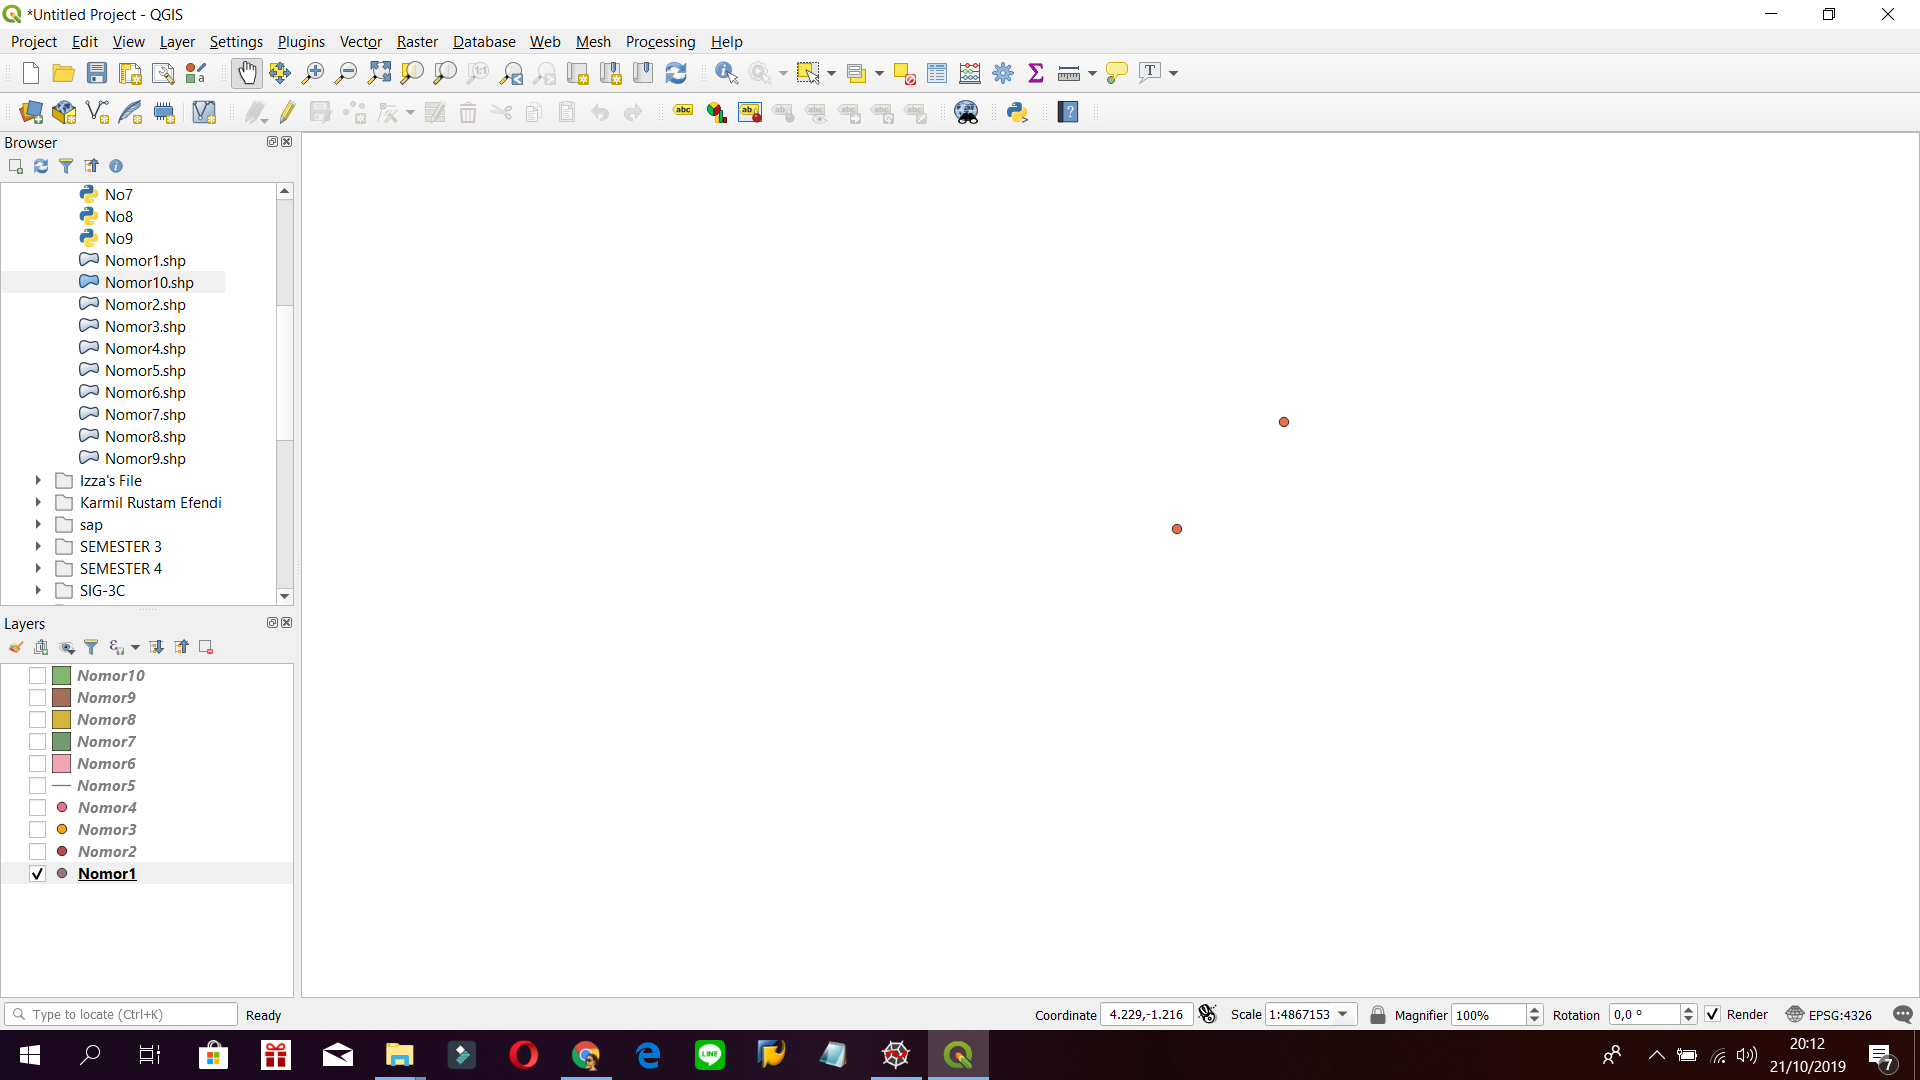
\includegraphics[width=6cm]{figures/Tugas2/1174053/no1.png}
		\centering
		\caption{Point (Titik)}
	\end{figure}
	
	\item Nomor 2
	\lstinputlisting{src/tugas2/1174053/No2.py}
	\begin{figure}[H]
		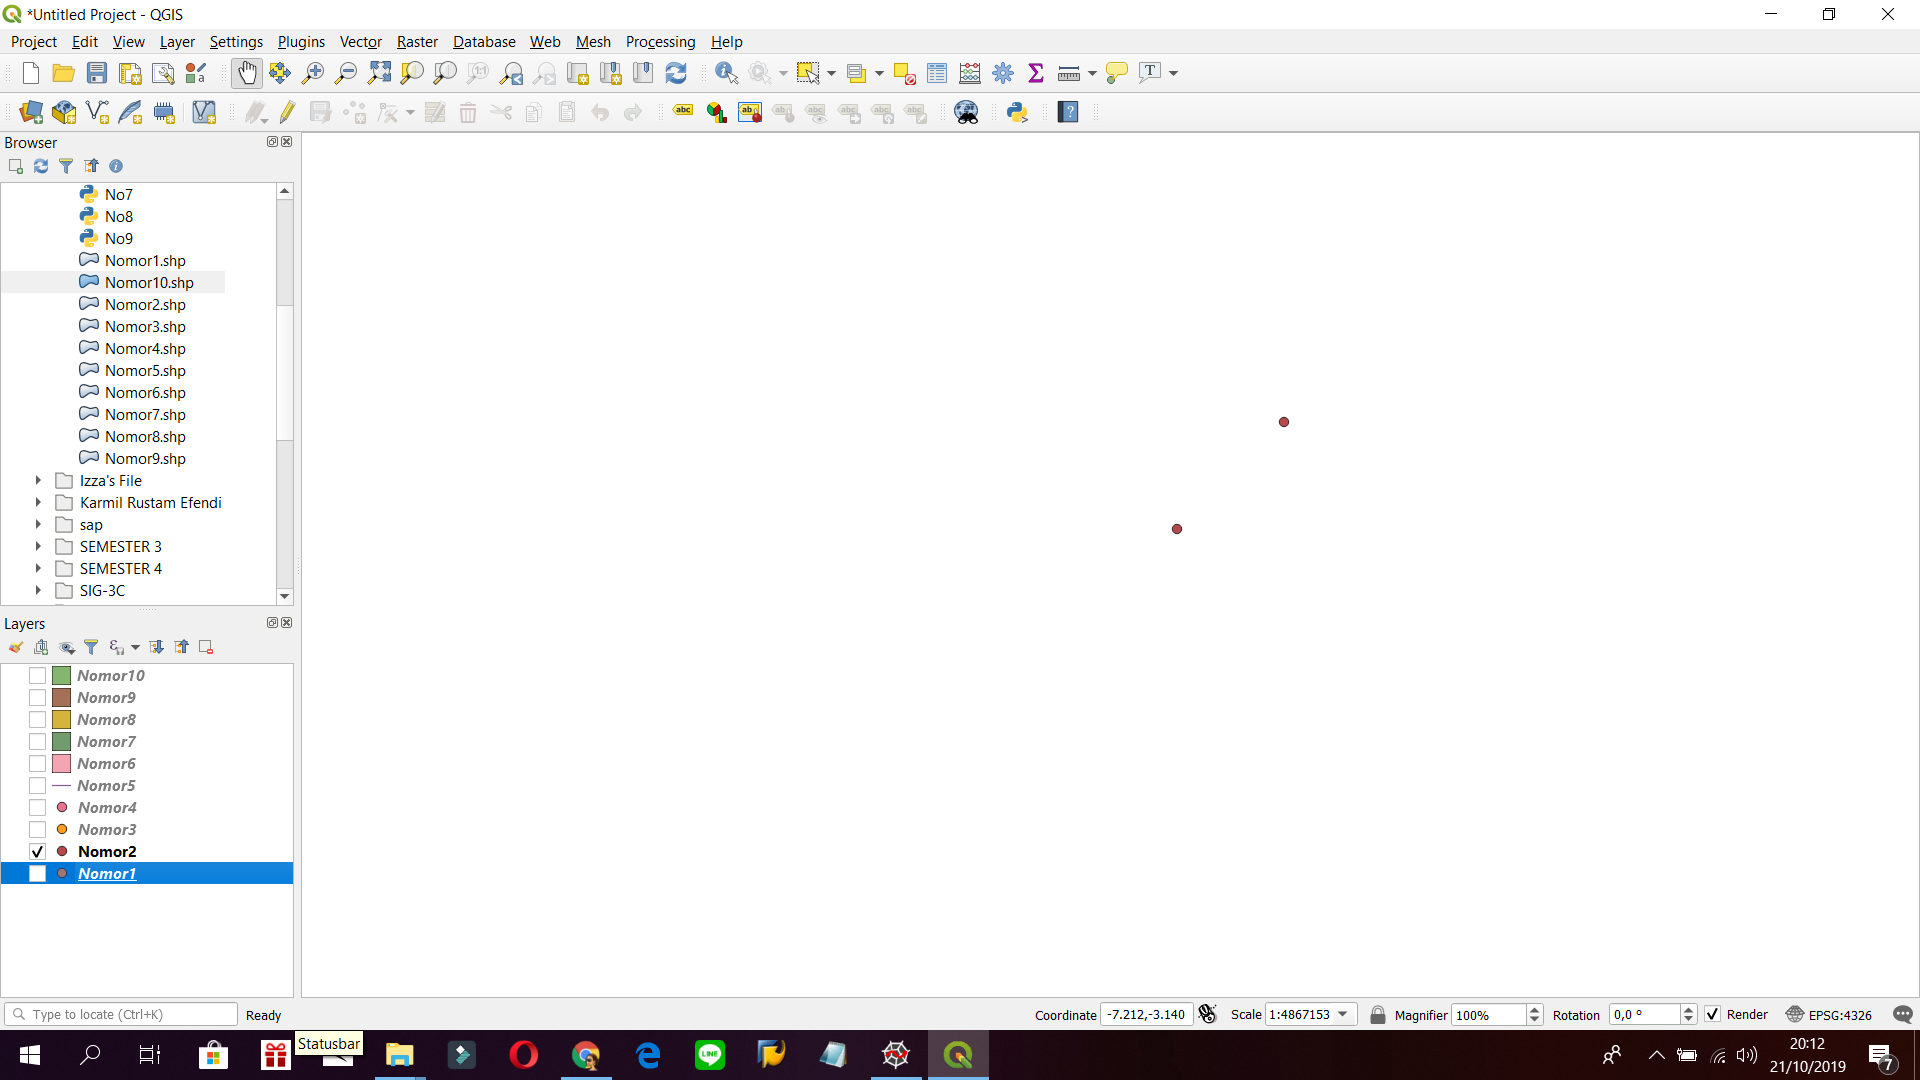
\includegraphics[width=6cm]{figures/Tugas2/1174053/no2.png}
		\centering
		\caption{Point (Titik)}
	\end{figure}

	\item Nomor 3
	\lstinputlisting{src/tugas2/1174053/No3.py}
	\begin{figure}[H]
		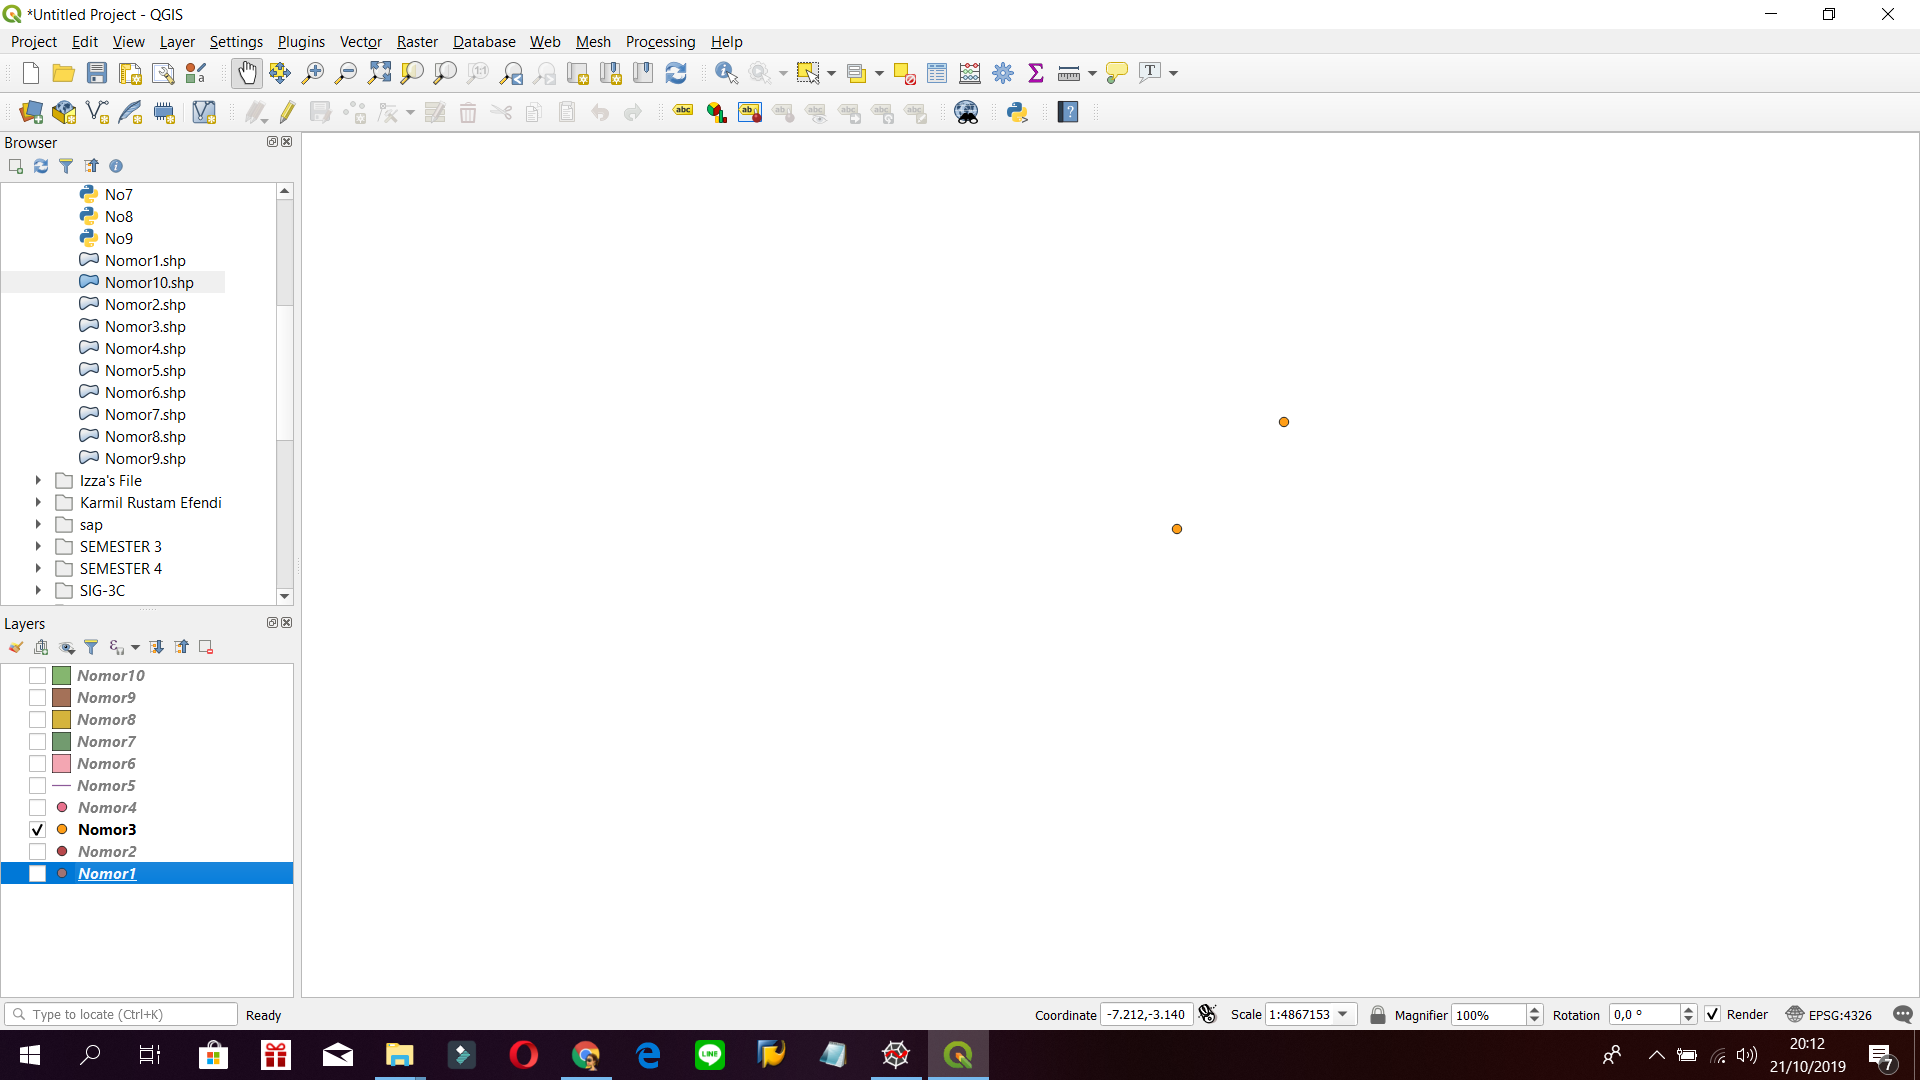
\includegraphics[width=6cm]{figures/Tugas2/1174053/no3.png}
		\centering
		\caption{Point (Titik)}
	\end{figure}
	
	\item Nomor 4
	\lstinputlisting{src/tugas2/1174053/No4.py}
	\begin{figure}[H]
		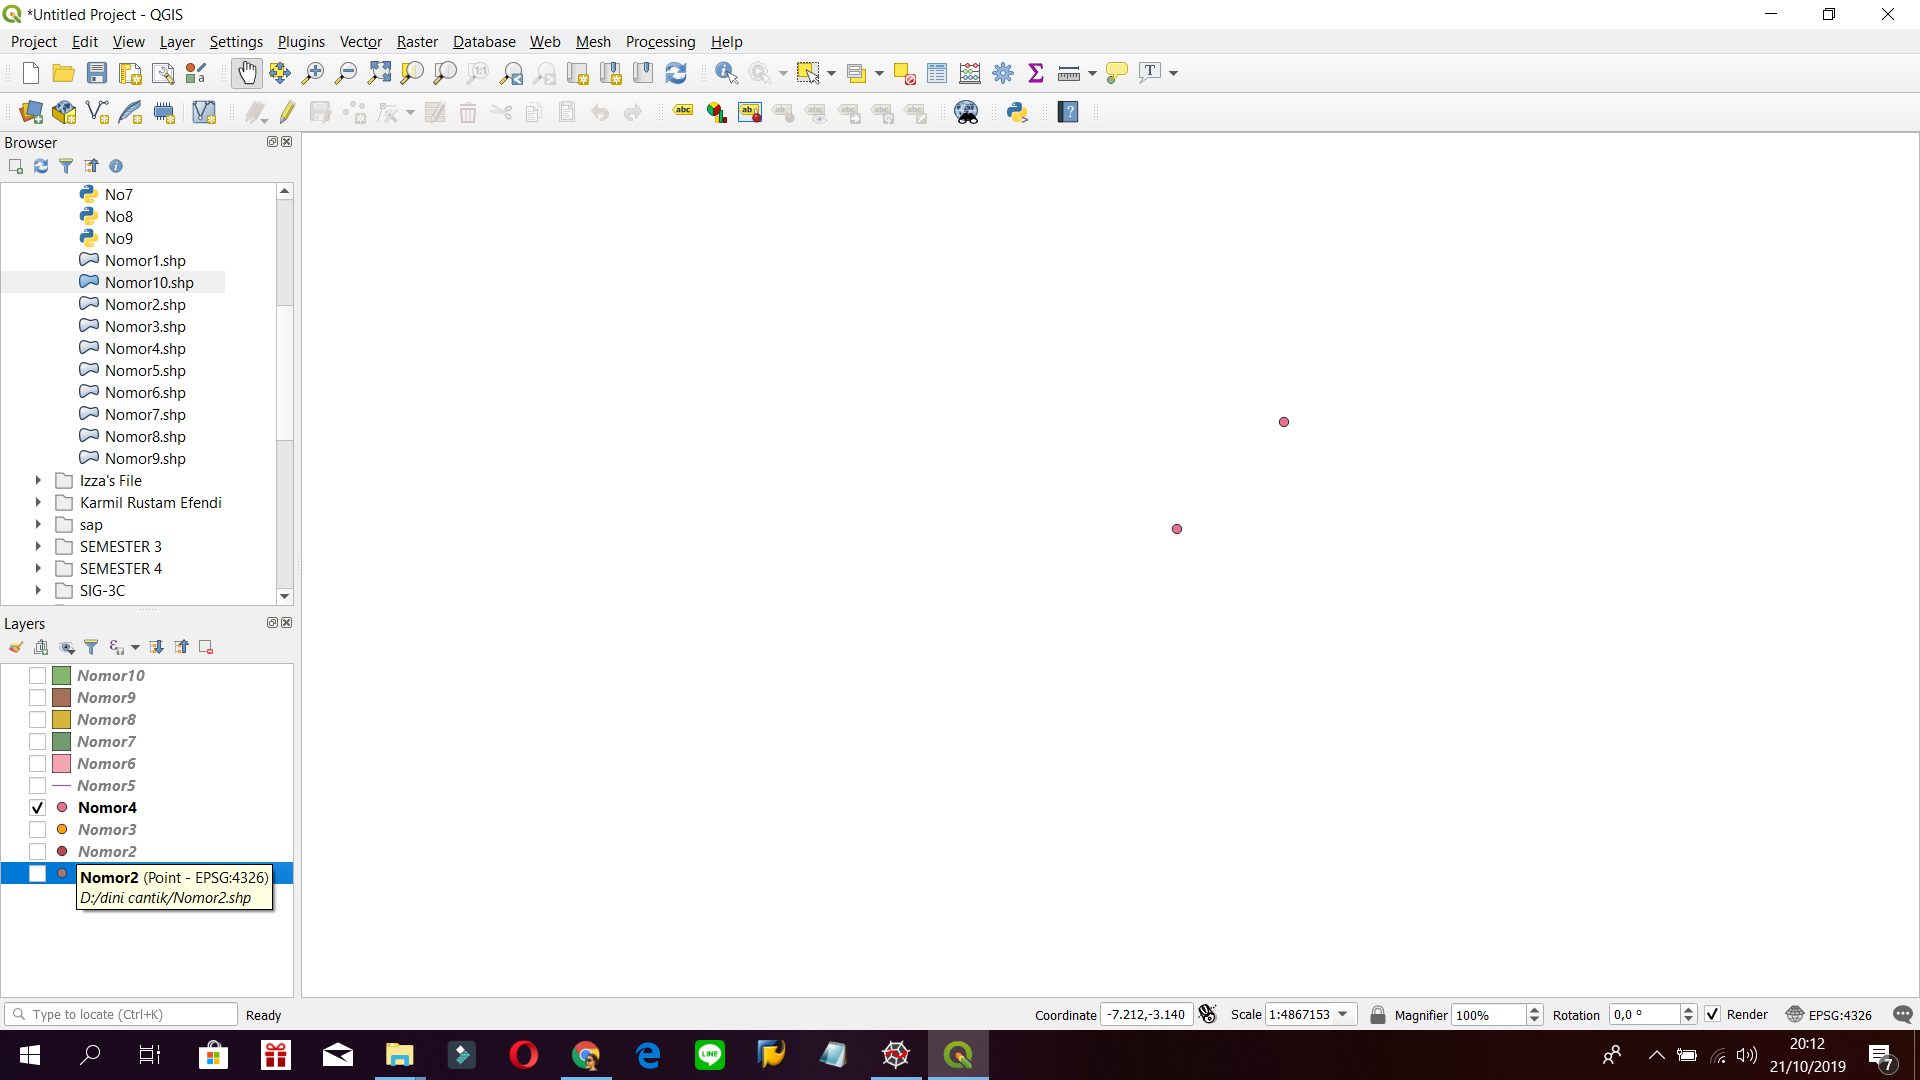
\includegraphics[width=6cm]{figures/Tugas2/1174053/no4.png}
		\centering
		\caption{Point (Titik)}
	\end{figure}
	
	\item Nomor 5
	\lstinputlisting{src/tugas2/1174053/No5.py}
	\begin{figure}[H]
		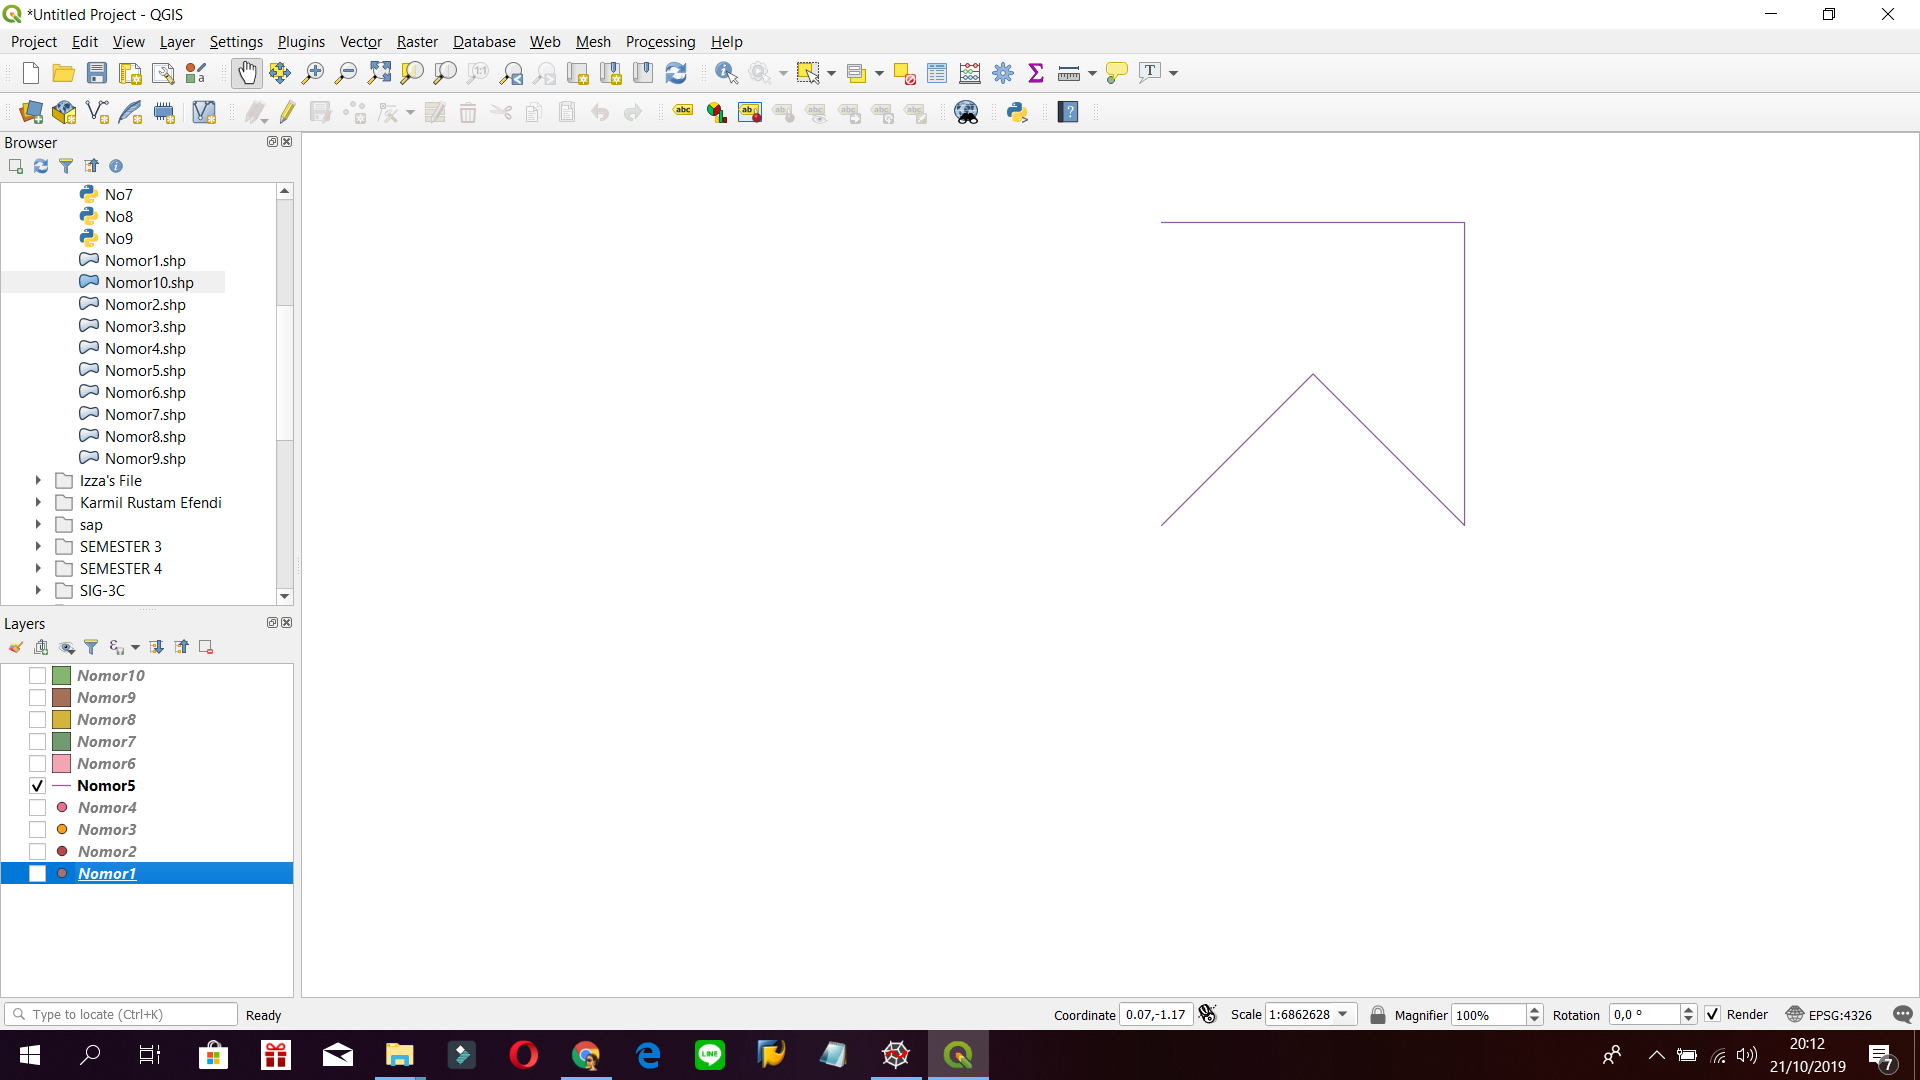
\includegraphics[width=6cm]{figures/Tugas2/1174053/no5.png}
		\centering
		\caption{PolyLine (Garis)}
	\end{figure}
	
	\item Nomor 6
	\lstinputlisting{src/tugas2/1174053/No6.py}
	\begin{figure}[H]
		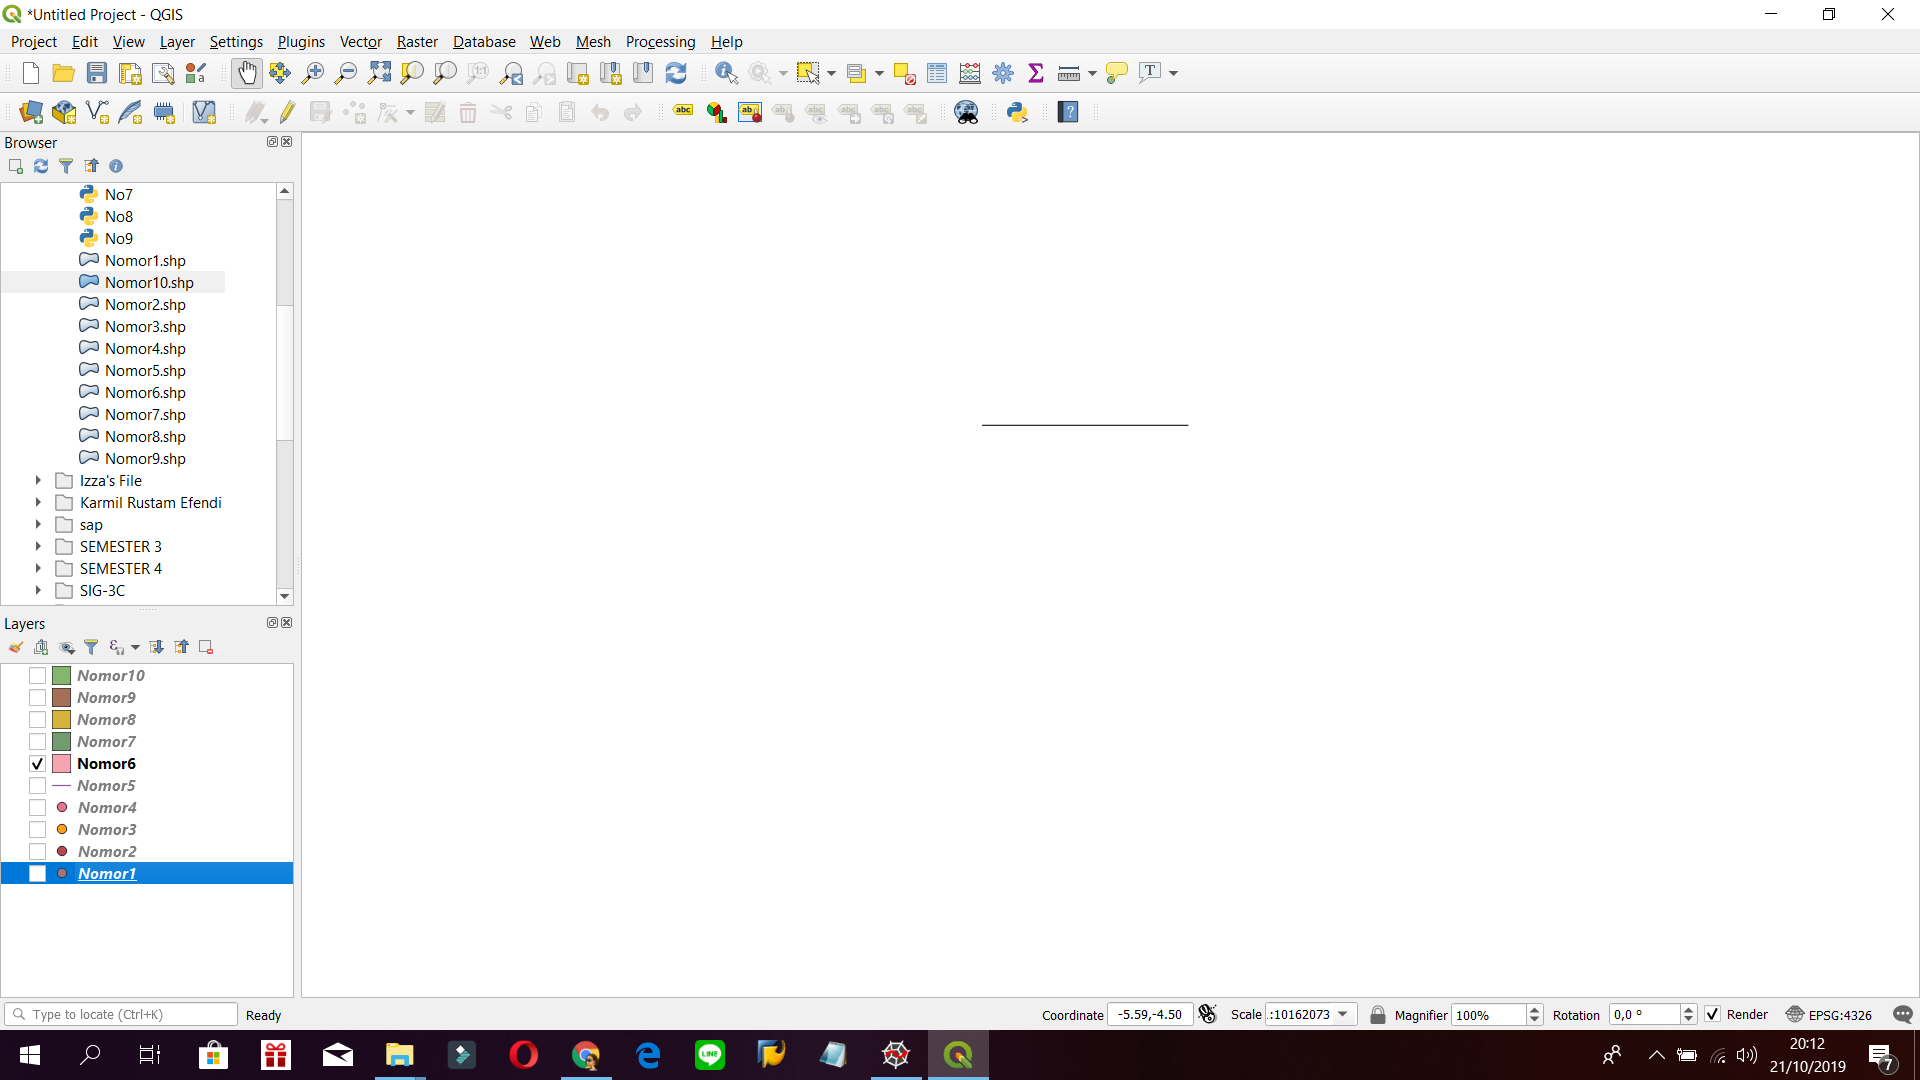
\includegraphics[width=6cm]{figures/Tugas2/1174053/no6.png}
		\centering
		\caption{Polygon (Bidang)}
	\end{figure}
	
	\item Nomor 7
	\lstinputlisting{src/tugas2/1174053/No7.py}
	\begin{figure}[H]
		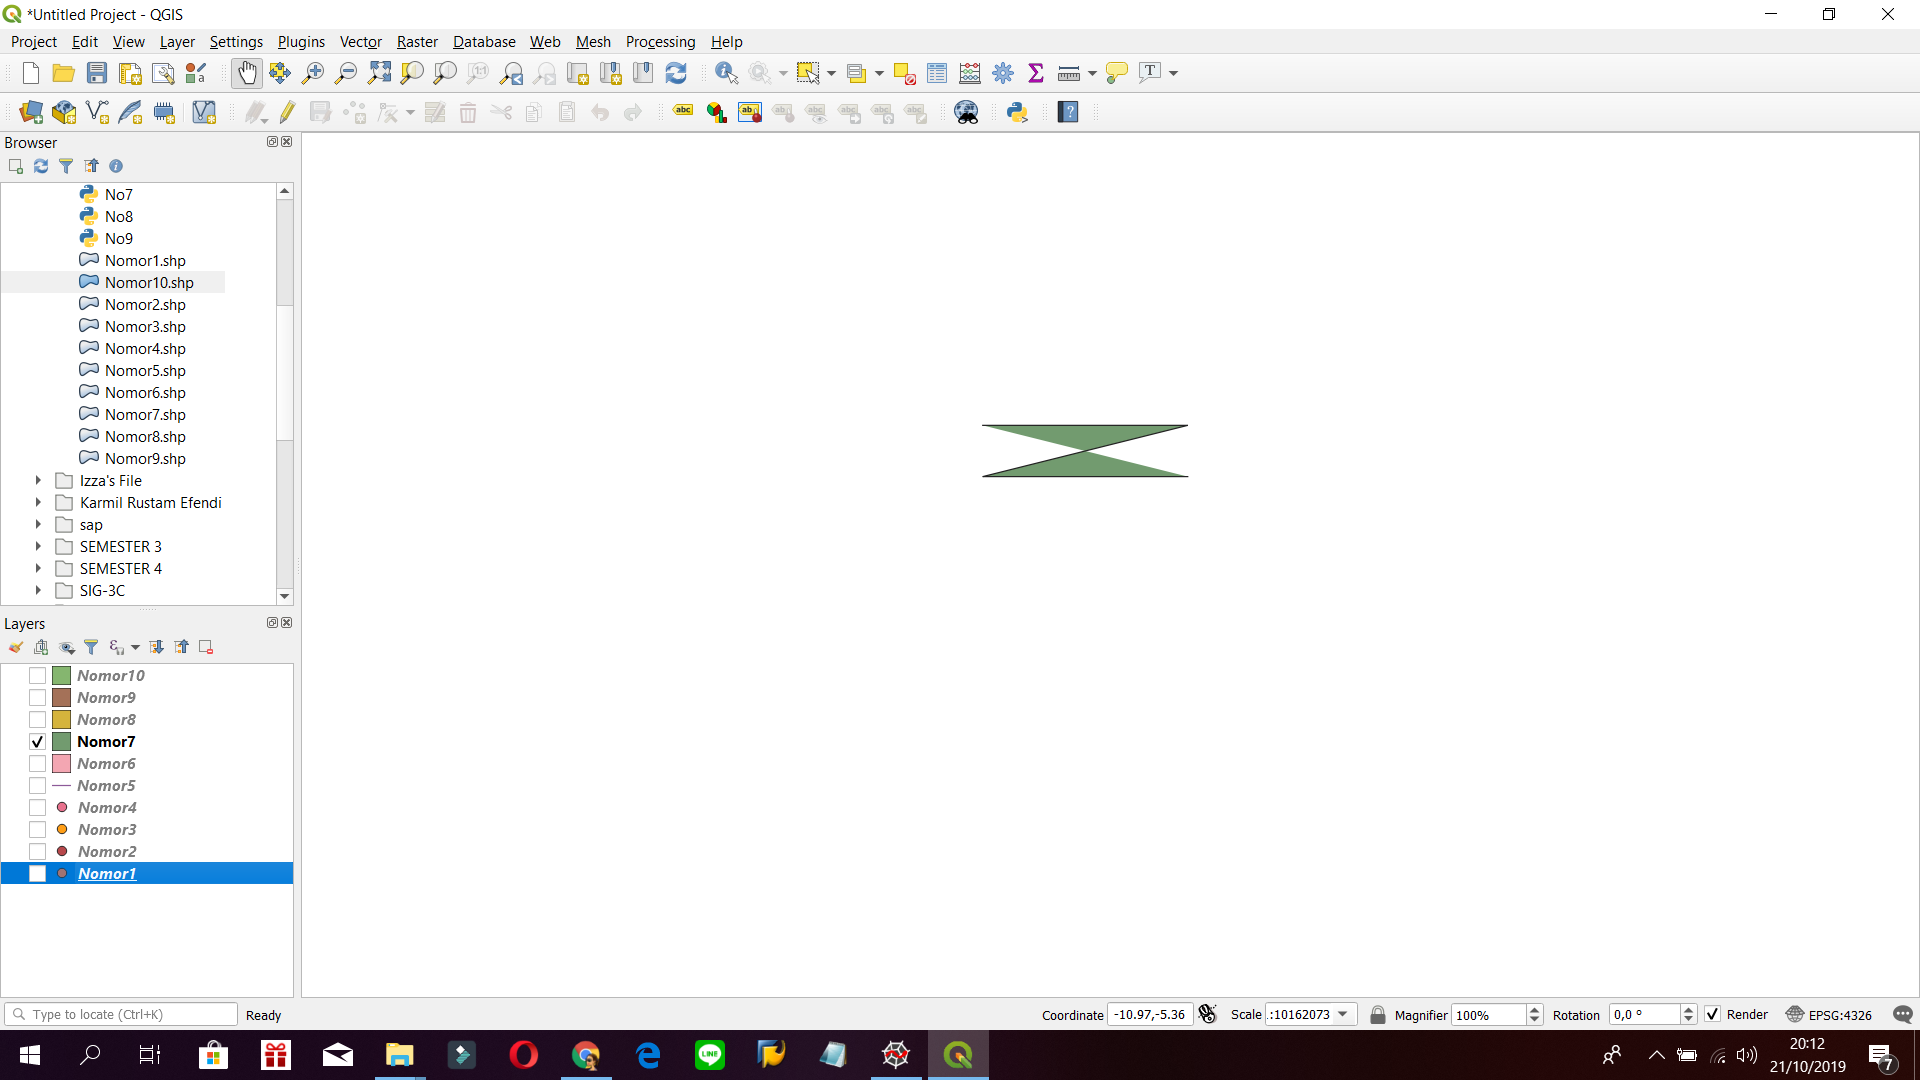
\includegraphics[width=6cm]{figures/Tugas2/1174053/no7.png}
		\centering
		\caption{Polygon (Bidang)}
	\end{figure}
	
	\item Nomor 8
	\lstinputlisting{src/tugas2/1174053/No8.py}
	\begin{figure}[H]
		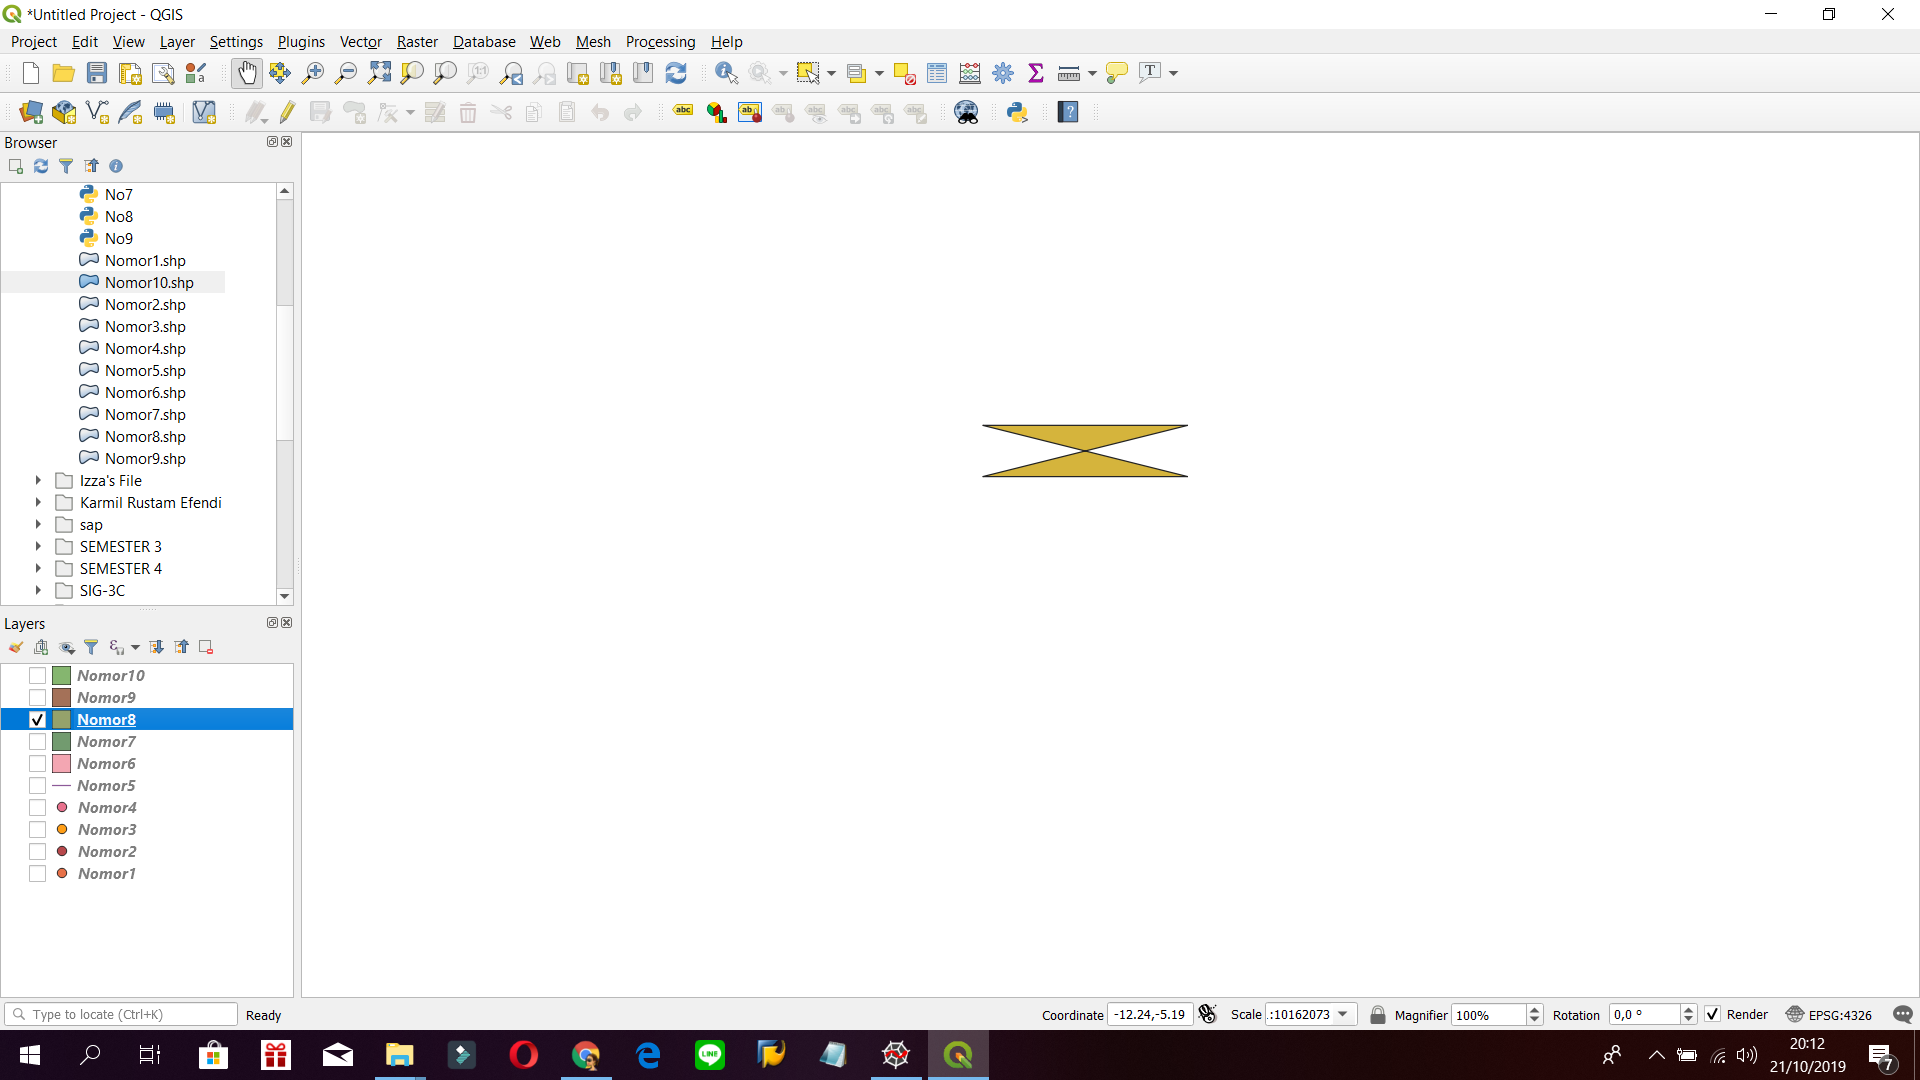
\includegraphics[width=6cm]{figures/Tugas2/1174053/no8.png}
		\centering
		\caption{Polygon (Bidang)}
	\end{figure}
	
	\item Nomor 9
	\lstinputlisting{src/tugas2/1174053/No9.py}
	\begin{figure}[H]
		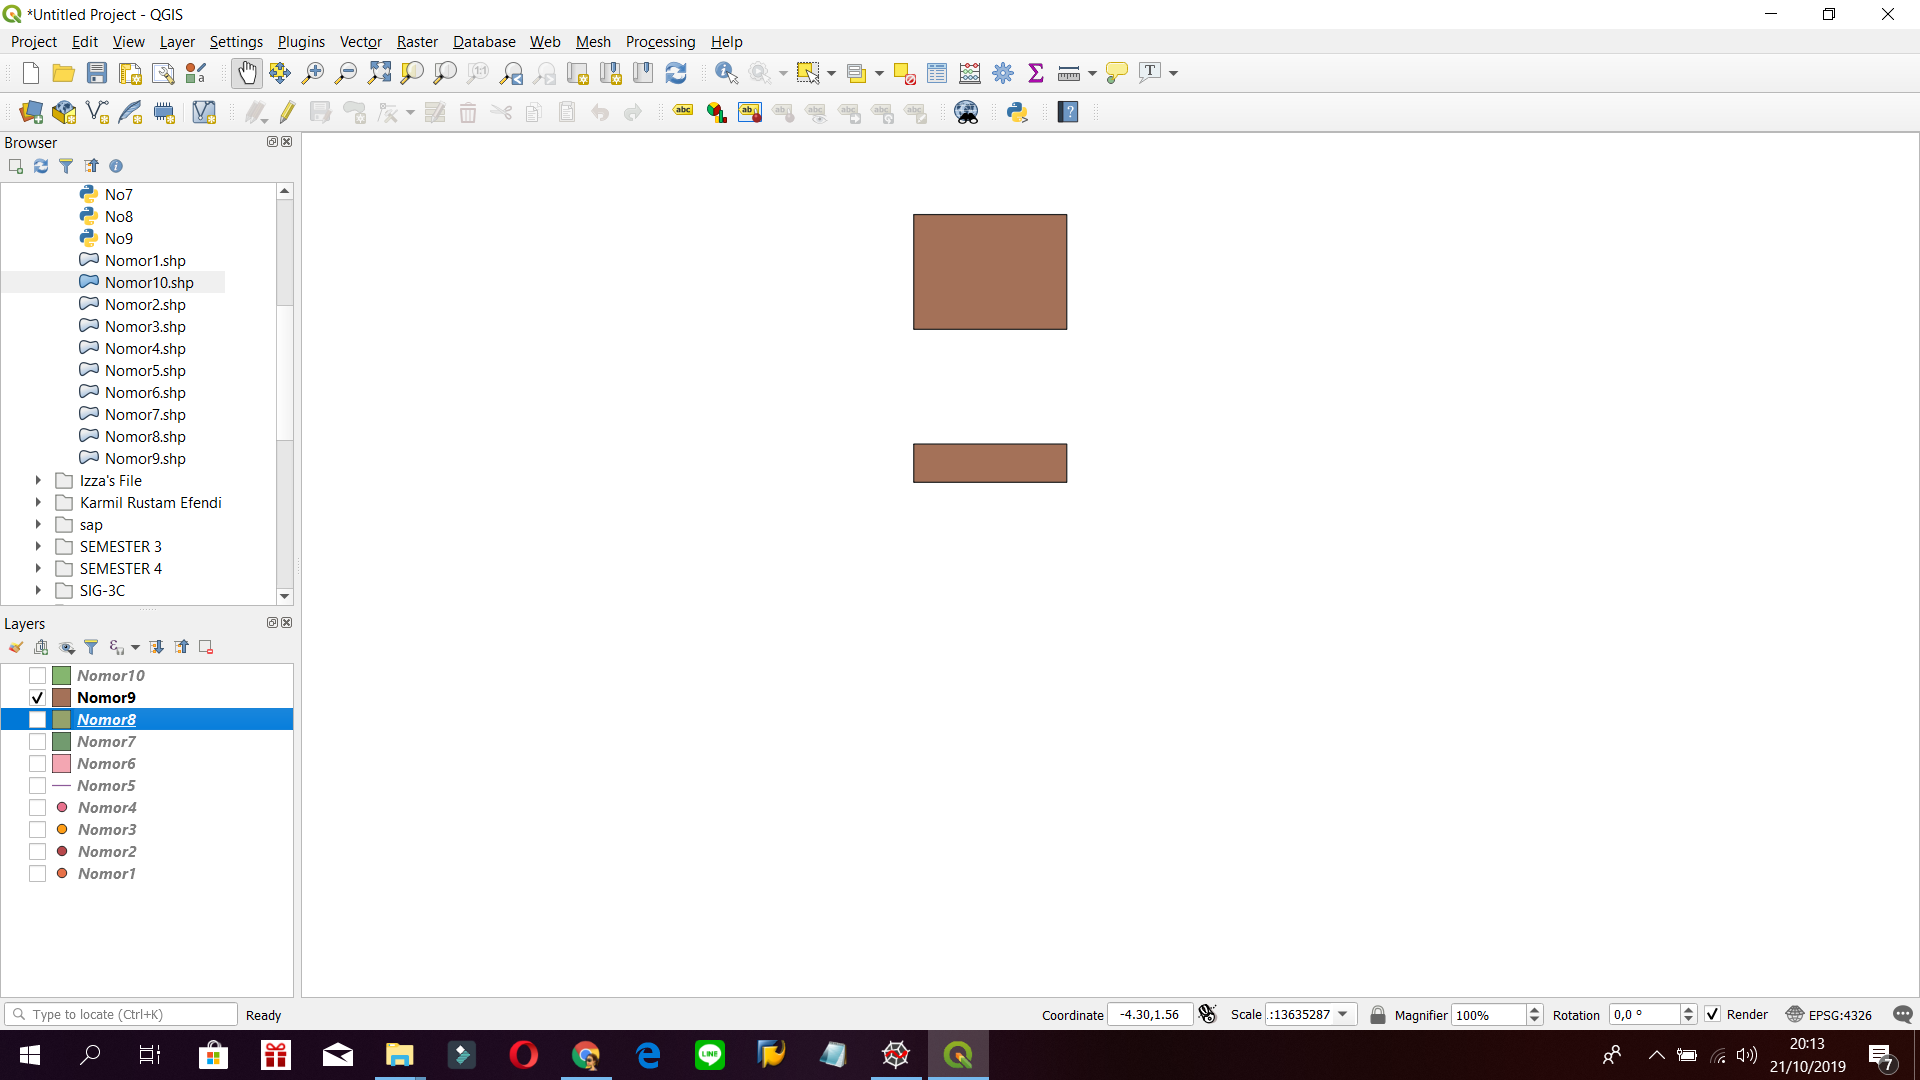
\includegraphics[width=6cm]{figures/Tugas2/1174053/no9.png}
		\centering
		\caption{Polygon (Bidang)}
	\end{figure}
	
	\item Nomor 10
	\lstinputlisting{src/tugas2/1174053/No10.py}
	\begin{figure}[H]
		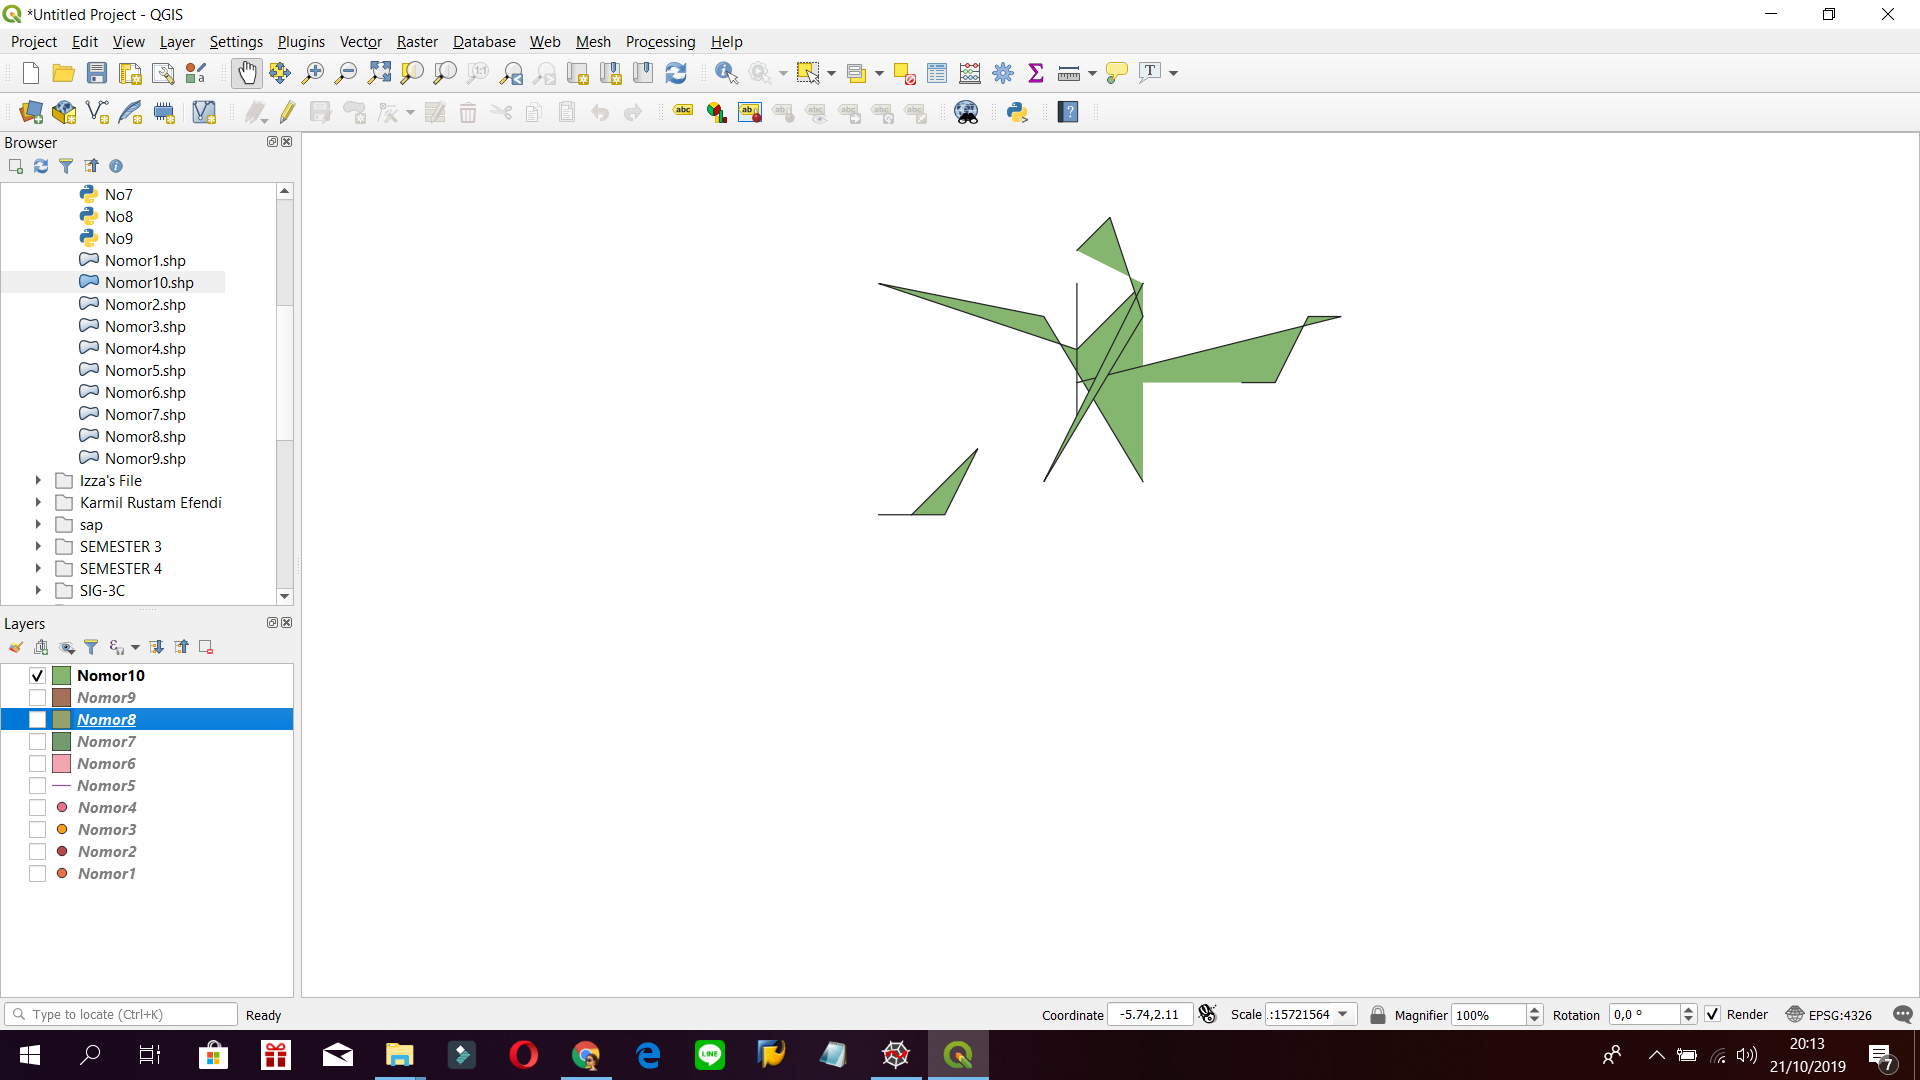
\includegraphics[width=6cm]{figures/Tugas2/1174053/no10.png}
		\centering
		\caption{Polygon, Hasil modulus dari npm saya 1174053} 
	\end{figure}
	
\end{enumerate}
\subsection{Link}
https://bit.ly/2P4RP6M
